\section{A Graphical Program Representation for Analysis and Optimization}
\label{sec:graph-representation}

For machine learning to successfully reason over programs, a suitable
input representation must be used. This section presents
\textsc{ProGraML}, a novel program representation that closely matches
the representations used traditionally within compilers and can be
processed natively by machine learning models. Unlike prior approaches
that rely on hand-engineered feature
extractors~\cite{Ashouri2018,Wang2018} or which are closely tied to
the syntax of the target program language~\cite{Allamanis2017b}, our
approach captures whole-program control, data, and call relations and
is both task- and language-agnostic.

\begin{figure*}
  \centering %
  \begin{subfigure}{.48\linewidth}%
    \centering
    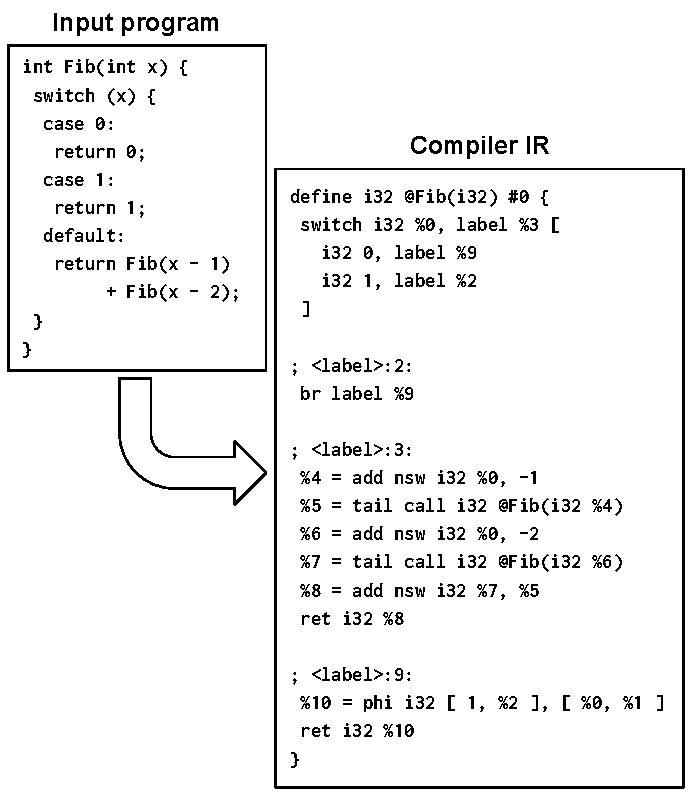
\includegraphics[width=\linewidth]{images/A_IR}%
    \caption{Compiler intermediate representation.}
    \label{subfigure:ir}%
  \end{subfigure}
  \begin{subfigure}{.48\linewidth}%
    \centering
    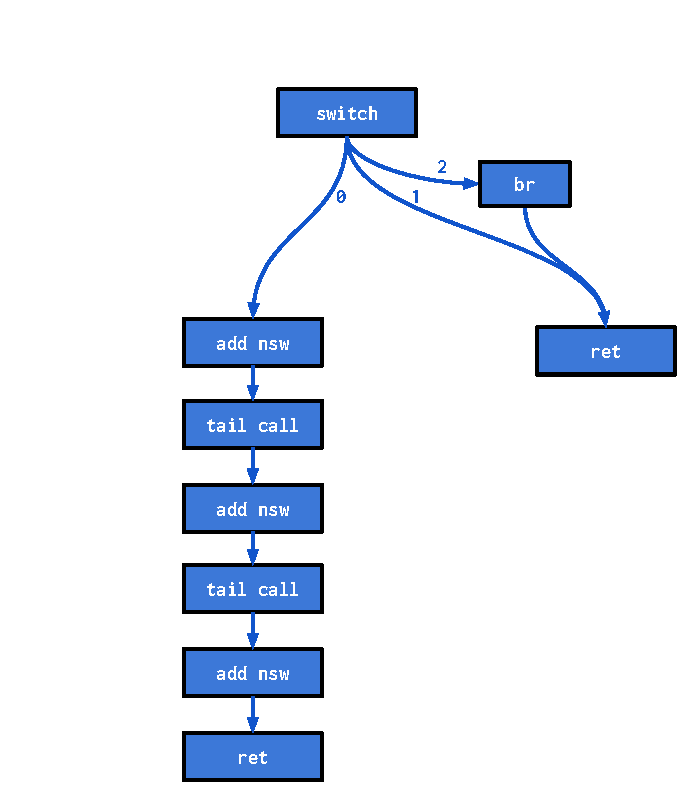
\includegraphics[width=\linewidth]{images/B_Control}%
    \caption{Construct control flow.}
    \label{subfigure:control_flow}%
  \end{subfigure}
  \\*
  \vspace{1em}
  \begin{subfigure}{.48\linewidth}%
    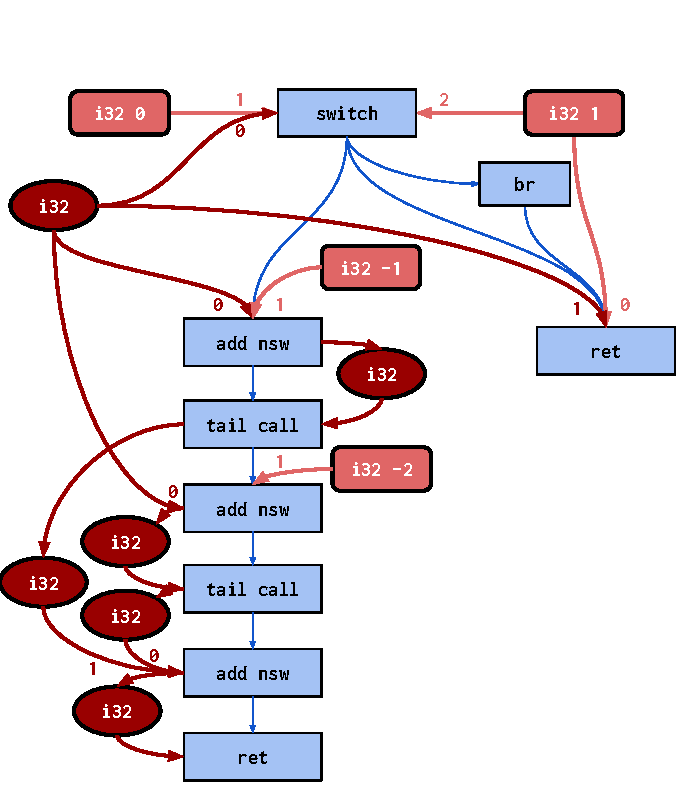
\includegraphics[width=\linewidth]{images/C_Data}%
    \caption{Add data flow for variables and constants.}
    \label{subfigure:data_flow}%
  \end{subfigure}
  \begin{subfigure}{.48\linewidth}%
    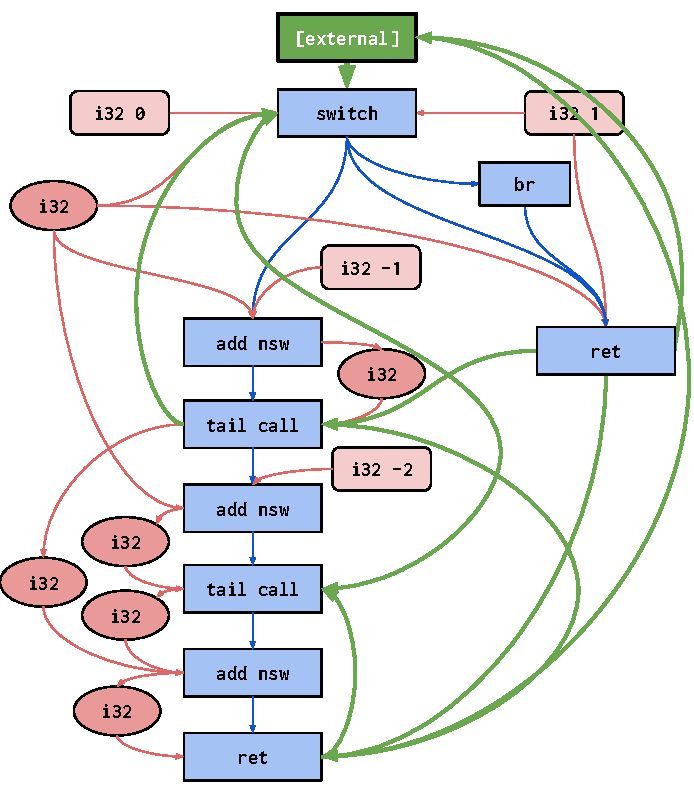
\includegraphics[width=\linewidth]{images/D_Call}%
    \caption{Add call flow for call sites.}
    \label{subfigure:call_flow}%
  \end{subfigure}
  \caption{%
    Construction of a \textsc{ProGraML} representation for a simple C
    implementation of recursive Fibonacci using LLVM-IR. The input
    program is passed through the compiler front end to produce an
    intermediate representation (a). A full flow graph is constructed
    from the IR statements and control flow edges inserted
    (b). Vertices for variables and constant values are  added and
    data-flow edges inserted (c). Finally, call sites are extracted
    and call edges inserted from call sites to function entry
    statements, and from function exit vertices to call sites (d). All
    edges are positional, for clarity we have omitted position labels
    where not required.%
  }%
  \label{figure:graph_construction}%
\end{figure*}

\subsection{Overview}

The \textsc{ProGraML} representation of a compiler IR serves as the
union between a call graph, control-flow graph, and data-flow
graph. We represent programs as directed multigraphs where statements,
identifiers, and immediate values are vertices, and relations between
vertices are edges. Edges are typed to differentiate control-, data-,
and call-flow. Additionally, we augment edges with a positional label
to encode the order of operands for statements, and to differentiate
between divergent branches in control-flow. The \textsc{ProGraML}
representation is processed natively by our machine learning models,
described in Section~\ref{sec:graph-based-machine-learning}.

\subsection{Graph Construction}

We construct a \textsc{ProGraML} graph $G = (V, E)$ by traversing a
compiler IR. Graph construction is divided into three stages:
control-flow, data-flow, and call-flow, though in practice the three
stages can be combined in a single $\bigo{(|V|+|E|)}$ pass. The
representation is compiler-agnostic, adding support for a new compiler
requires only a parser for the IR. Currently we support
LLVM~\cite{Lattner2004} and XLA HLO~\cite{Leary2017}
IRs. Figure~\ref{figure:graph_construction} shows the graph
construction approach.

\paragraph{(I) Control Flow} We construct a full-flow graph from an IR
by inserting a graph vertex for each instruction and control flow
edges between them, as shown in
Figure~\ref{subfigure:control_flow}. All control edges are augmented
with a numeric position label using an ascending sequence based on
their order in the list of a vertex's outgoing control edges. For
instructions with a single control successor, the position of the
control edge is 0. For a branching statement with $n$ successor
statements, the control edge positions are in the range
$0 \le e_{\text{pos}} \le n$. We do not need to encode the source
function or basic block~\cite{Lattner2004} of instructions as this
information is captured implicitly in structure of the graph; basic
blocks are regions of instructions with a single entry and exit
control edge, and functions are disconnected subgraphs.

\paragraph{(II) Data Flow} We introduce additional graph vertices for
constant values and variables, shown in
Figure~\ref{subfigure:data_flow}. Data-flow edges are added to capture
the relation from constants and variables to the instructions that use
them as operands, and instructions to produced variables. Each unique
variable and constant is a vertex, which implicitly models the scope
of variables, and unlike the tokenized representations of prior
machine learning works, variables in different scopes always map to
distinct vertices and can thus be discerned. Similarly, constant
values with the same textual representation in source code (such as
the number \texttt{3.14} with \texttt{float} and \texttt{double}
precision types) are distinguishable in our representation. As with
control edges, data edges have a position label which encodes the
order of operands for instructions. The latent representation of an IR
statement is thus a function of the vertex representing the
instruction and the vertices of any operand variables or constants,
modulated by their order in the list of operands.

\paragraph{(III) Call Flow} Control edges do not span functions, such
that an IR with functions $F$ produces $|F|$ disconnected subgraphs
(the same is not true for data edges which may cross function
boundaries, for example in the case of an global constant which is
used within multiple functions of a program). Instead, the relation
between a statement which calls a function and the called function is
captured through call edges, shown in
Figure~\ref{subfigure:call_flow}. An outgoing call edge is inserted
from the calling statement to the entry statement of a
function. Return call edges are added from all terminal statements of
a function to the calling statement. Call edges do not use position
labels as there is no ordering to be imposed between the call sites of
a function. For IRs which support external linkage, an additional
vertex is created representing an external callsite and connected to
all externally visible functions. Similarly, if a call site references
a function not defined in the current IR, a \emph{dummy} function
definition is created consisting of a pair of entry and exit
instruction vertices, and connected normally through call edges. A
single dummy function definition is created for each externally
defined function and shared across all call sites in the current IR.


\subsection{Comparison to Other Representations}

As an input for machine learning, what distinguishes \textsc{ProGraML}
from prior works is its close proximity to the structured
representations traditionally used within compilers for program
analysis and optimization. Specifically, it is distinct from prior
machine learning representations in three key areas:
\begin{enumerate}
\item as an IR-level representation, it is independent of the source
  language and accompanying variances such as code style and
  identifier naming that affect source-level
  representations~\cite{Alon2018a,Cummins2017a};
\item by representing programs as graphs with explicit control, data,
  and call edge types \textsc{ProGraML} captures a greater range of
  intra-program relations than prior graph
  representations~\cite{Ben-nun2018,Allamanis2017b,Park2012};
\item and in trading sequential for graph representations, we do not
  sacrifice local sequence order, such as the ordering of diverging
  control flow or the ordering of operands that is lost in prior
  representations~\cite{Ben-nun2018,Brauckmann2020}.
\end{enumerate}

Table~\ref{tab:representation_taxonomy} provides a comparison of
\textsc{ProGraML} to several recent learned representations of code.

\begin{table}
  \centering
  \footnotesize
  \begin{tabular}{r L{3.6cm} L{2.5cm} L{1.8cm} L{1.8cm} L{1.8cm}}
    \toprule
    & Source Languages & Representation & Flow-sensitive? & Position-sensitive? & Value-sensitive? \\
    \midrule
    AST Paths~\cite{Alon2018c} & C\#, Java, JavaScript, Python & AST & &  & \cmark \\
    CDFG~\cite{Brauckmann2020} & OpenCL & IR Graph & \cmark &  &  \\
    code2vec~\cite{Alon2018a} & Java & AST & & & \cmark \\
    DeepTune~\cite{Cummins2017b} & OpenCL & Token Sequence &  & \cmark & \cmark \\
    DeepTune-IR\cite{Barchi2019a} & OpenCL & IR Token Sequence &  & \cmark & \\
    DeepTyper~\cite{Hellendoorn2018} & JavaScript & Token Sequence &  & \cmark & \cmark \\
    inst2vec~\cite{Ben-nun2018} & C++, OpenCL & IR Graph & \cmark & & \cmark \\
    \textbf{\textsc{ProGraML}} & \textbf{C, C++, Fortran, Haskell, OpenCL, Swift} & \textbf{IR Graph} & \cmark & \cmark & \cmark \\
    \bottomrule
  \end{tabular}
  \vspace{.3em}
  \caption{%
    Taxonomy of recent code representations for machine learning. We
    classify approaches based on the type of representation used and
    the sensitivity to three categories: \{control/data/call\}-flow,
    operand positions, and operand values. Prior approaches require a
    trade-off in representational power, e.g. substituting a
    position-sensitive token sequence for a flow-sensitive
    graph. \textsc{ProGraML} is the first representation to span all
    categories.%
  }%
  \label{tab:representation_taxonomy}
\end{table}
